%\documentclass[msc]{on} %para dissertação de mestrado, descomentar esta linha e comentar a de baixo
\documentclass[dsc]{on}
%\documentclass[msc, numbers]{on} %a opção numbers da classe, mostrada nesta linha, é usada para citação por lista numérica em ordem de ocorrência
\usepackage[utf8]{inputenc}
\usepackage{amsmath,amssymb}
\usepackage{hyperref}

%pacotes utilizados
\usepackage{enumerate} %para gerar listas numeradas
\usepackage{graphicx}  %para figuras eps
\usepackage{subfigure} %para figuras múltimas, com (a), (b), (c), etc.

\makelosymbols
\makeloabbreviations

\begin{document}
  \title{Título da Tese ou Dissertação}
  \foreigntitle{Thesis Title}
  \author{Nome do Autor}{Sobrenome}
  \advisor{Prof.}{Nome do Orientador}{Sobrenome}{D.Sc.}
% Comente a linha abaixo se não houver coorientador
  \coadvisor{Prof.}{Nome do Primeiro Co-orientador}{Sobrenome}{D.Sc.}
%  \coadvisor{Prof.}{Nome do Segundo Co-orientador}{Sobrenome}{Ph.D.}
%  \coadvisor{Prof.}{Nome do Terceiro Co-orientador}{Sobrenome}{D.Sc.}


  \examiner{Prof.}{Nome do Primeiro Examinador Sobrenome}{D.Sc.}
  \examiner{Prof.}{Nome da Segunda Examinadora Sobrenome}{Ph.D.}
  \examiner{Dr.}{Nome da Terceira Examinadora Sobrenome}{D.Sc.}
  \examiner{Prof.}{Nome do Quarto Examinador Sobrenome}{Ph.D.}
  \examiner{Prof.}{Nome do Quinto Examinador Sobrenome}{Ph.D.}
  \department{COGE}
  \date{05}{2014}

  \keyword{Primeira palavra-chave}
  \keyword{Segunda palavra-chave}
  \keyword{Terceira palavra-chave}

  \maketitle

  \frontmatter
  \dedication{Dedicat\'oria (opcional).}


  \chapter*{Agradecimentos}

Agradecimentos (opcional).

  \begin{abstract}

Apresenta-se, nesta tese, ...

\end{abstract}


  \begin{abstract}

Apresentamos avanços metodológicos na área de modelagem direta e inversão
regional de dados de gravimetria por satélite.
Com esse fim, desenvolvemos dois projetos \DIFdelbegin \DIFdel{de software }\DIFdelend \DIFaddbegin \DIFadd{computacionais }\DIFaddend de código livre.
O primeiro é um conjunto de programas de linha de comando feitos na linguagem C
chamado \textit{Tesseroids}.
Os programas calculam o potencial, aceleração e tensor gradiente gravitacional
de um prisma esférico, ou tesseroide.
\textit{Tesseroids} implementa e aprimora um algoritmo de discretização
adaptativa para automaticamente garantir a acurácia das computações.
\DIFdelbegin \DIFdel{Nossos }\DIFdelend \DIFaddbegin \DIFadd{Os }\DIFaddend resultados com testes numéricos mostram que, para obter o mesmo nível de
acurácia, a aceleração gravitacional demanda uma discretização mais fina que o
potencial.
Por sua vez, o tensor gradiente gravitacional demanda discretização mais fina
ainda que a aceleração.
O segundo \DIFdelbegin \DIFdel{software }\DIFdelend \DIFaddbegin \DIFadd{projeto computacional }\DIFaddend é o \textit{Fatiando a Terra}, uma biblioteca
feita na linguagem Python para inversão, modelagem direta, processamento e
visualização de dados.
A biblioteca permite que o usuário combine as ferramentas de modelagem direta e
\DIFaddbegin \DIFadd{de }\DIFaddend inversão para implementar novos métodos de inversão.
As ferramentas de modelagem direta incluem uma implementação do algoritmo
utilizado no programa \textit{Tesseroids}.
\DIFdelbegin \DIFdel{Nós combinamos }\DIFdelend \DIFaddbegin \DIFadd{Combinamos }\DIFaddend os recursos de inversão e modelagem direta com tesseroides do
\textit{Fatiando a Terra} para desenvolver um método rápido para a inversão
não-linear de dados de gravidade.
O método estima a profundidade da interface crosta-manto (a Moho) baseado em
dados de gravidade utilizando uma aproximação esférica da Terra.
\DIFdelbegin \DIFdel{Nós adaptamos }\DIFdelend \DIFaddbegin \DIFadd{Adaptamos }\DIFaddend o método de Bott, que é computacionalmente eficiente, para
incluir regularização de suavidade  e utilizar tesseroides ao invés de prismas
retangulares retos.
A inversão é controlada por três hiper-parâmetros: o parâmetro de
regularização, o contraste de densidade \DIFdelbegin \DIFdel{na Moho }\DIFdelend \DIFaddbegin \DIFadd{entre a Terra real e o modelo de
referência (a Terra Normal) }\DIFaddend e a profundidade da Moho \DIFdelbegin \DIFdel{de
referência.
Nós aplicamos }\DIFdelend \DIFaddbegin \DIFadd{da Terra Normal.
Aplicamos }\DIFaddend dois tipos de validação cruzada para estimar esses parâmetros de
maneira automática.
Testes com dados sintéticos confirmam a capacidade do método proposto de
estimar os três hiper-parâmetros e o relevo suave da Moho.
\DIFdelbegin \DIFdel{Por fim, nós aplicamos nosso }\DIFdelend \DIFaddbegin \DIFadd{Finalmente, aplicamos o }\DIFaddend método de inversão \DIFaddbegin \DIFadd{desenvolvido }\DIFaddend para gerar um modelo de
profundidade da Moho para a América do Sul.
\DIFdelbegin \DIFdel{Nosso modelo }\DIFdelend \DIFaddbegin \DIFadd{O modelo de profundidade da Moho estimado }\DIFaddend ajusta os dados de gravidade
observados e \DIFaddbegin \DIFadd{as }\DIFaddend estimativas da profundidade da Moho provenientes da sismologia nas
regiões oceânicas e nas partes central e \DIFdelbegin \DIFdel{Leste }\DIFdelend \DIFaddbegin \DIFadd{leste }\DIFaddend do continente.
\DIFdelbegin \DIFdel{Nós observamos }\DIFdelend \DIFaddbegin \DIFadd{Observamos }\DIFaddend desajustes aos dados na região dos Andes, onde a profundidade da
Moho é a maior do continente.
Nas bacias do Amazonas, Solimões e Paraná, o modelo ajusta os dados de
gravidade mas não as estimativas da sismologia.
Essas discrepâncias indicam a presença de anomalias de densidade na crosta ou
manto superior, como sugerido anteriormente na literatura.
\end{abstract}

\begin{foreignabstract}

We present methodological improvements to forward modeling and regional
inversion of satellite gravity data.
For this purpose, we developed two open-source software projects.
The first is a C language suite of command-line programs called
\textit{Tesseroids}.
The programs calculate the gravitational potential, acceleration, and gradient
tensor of a spherical prism, or tesseroid.
\textit{Tesseroids} implements and extends an adaptive discretization algorithm
to automatically ensure the accuracy of the computations.
Our numerical experiments show that, to achieve the same level of accuracy, the
gravitational acceleration components require finner discretization than the
potential.
In turn, the gradient tensor requires finner discretization still than the
acceleration.
The second open-source project is \textit{Fatiando a Terra}, a Python language
library for inversion, forward modeling, data processing, and visualization.
The library allows the user to combine the forward modeling and inversion tools
to implement new inversion methods.
The gravity forward modeling tools include an implementation of the
algorithm used in the \textit{Tesseroids} software.
We combined the inversion and tesseroid forward modeling utilities of
\textit{Fatiando a Terra} to develop a new method for fast non-linear gravity
inversion.
The method estimates the depth of the crust-mantle interface (the Moho) based
on observed gravity data using a spherical Earth approximation.
We extended the computationally efficient Bott's method to include smoothness
regularization and use tesseroids instead right rectangular prisms.
The inversion is controlled by three hyper-parameters: the regularization
parameter, the \DIFdelbegin \DIFdel{Moho }\DIFdelend density-contrast \DIFaddbegin \DIFadd{between the real Earth and the reference model
(the Normal Earth)}\DIFaddend , and the depth of the \DIFdelbegin \DIFdel{reference Moho }\DIFdelend \DIFaddbegin \DIFadd{Moho of the Normal Earth}\DIFaddend .
We employ two cross-validation procedures to automatically estimate these
parameters.
Tests on synthetic data confirm the capability of the proposed method to
estimate smoothly varying Moho depths and the three hyper-parameters.
Finally, we applied \DIFdelbegin \DIFdel{our inversion method }\DIFdelend \DIFaddbegin \DIFadd{the inversion method developed }\DIFaddend to produce a Moho depth
model for South America.
\DIFdelbegin \DIFdel{Our }\DIFdelend \DIFaddbegin \DIFadd{The estimated Moho depth }\DIFaddend model fits the gravity data and seismological Moho
depth estimates in the oceanic areas and the central and eastern portions of
the continent.
We observe large misfits in the Andes region, where Moho depth is largest.
In Amazon, Solimões, and Paraná Basins, the model fits the observed gravity
but disagrees with seismological estimates.
These discrepancies suggest the existence of density-anomalies in the crust or
upper mantle, as has been suggested in the literature.
\end{foreignabstract}

  \tableofcontents
  \listoffigures
  \listoftables
  \printlosymbols
  \printloabbreviations

  \mainmatter
  \chapter{Introdução}

\textbf{OBS0: Testado com o MikTex 2.9 em Windows, rodando o PDFLaTex para geração diretamente do PDF da tese (anexado como exemplo). Como editor, indicamos o WinEdt. Entretanto, este template pode ser rodado em qualquer editor de texto e também no sistema operacional Linux.}

OBS1: Segundo a norma de formatação de teses e disserta{\c c}\~oes do
Programa de Pós-graduação em Geofísica do Observatório Nacional (ON/MCTI)
é obrigatório que toda abreviatura deva ser definida na primeira vez que é
utilizada, mas não é obrigatório colocar uma lista de abreviações no preâmbulo.
Entretanto, é altamente indicado que se coloque uma lista de abreviação no
preâmbulo, com todas as abreviações utilizadas no trabalho, uma vez que isto
torna o texto mais claro.

EXEMPLO.

Um exemplo de utilização de abreviação é dado na seguir: O Método das Diferenças Finitas
(MDF\abbrev{MDF}{Método dos Diferenças Finitas}) é um dos métodos numéricos mais eficientes
para a resolução de equações diferenciais...

Repare que, na primeira vez que a abreviação ocorre no texto, basta utilizar o comando
``\verb|\abbrev|'' para descrever a abreviação, sendo tal abreviação colocada automaticamente
e uma listagem de abreviações no preâmbulo do texto.

Do mesmo modo, pode-se definir os símbolos com o comando ``\verb|\symbl|'', tal como o
conjunto dos números reais $\mathbb{R}$ e o conjunto vazio $\emptyset$.
\symbl{$\mathbb{R}$}{Conjunto dos n\'umeros reais}
\symbl{$\emptyset$}{Conjunto vazio}

Após isto, antes de compilar o código com pdflatex por exemplo, é necessário rodar o make index
para gerar as listas, por exemplo, através dos seguinte comandos na linha de comando:

\verb|makeindex -s on.ist -o thesis.lab thesis.abx|

\verb|makeindex -s on.ist -o thesis.los thesis.syx|


  \chapter{Contexto Geológico}

Para ilustrar a completa ades\~ao ao estilo de cita{\c c}\~oes e listagem de
refer\^encias bibliogr\'aficas, a Tabela~\ref{tab:citation} apresenta cita{\c
c}\~oes de alguns dos trabalhos, utilizando o estilo alfabético (default). Para
utilização do estilo numérico, deve-se utilizar a opção number da classe ON, ou seja,
basta usar \verb|\documentclass[dsc, numbers]{on}|.

\begin{table}[h]
\caption[Exemplos de tabela (texto do índice)]{Exemplos de tabela mostrando os comandos para
  cita{\c c}\~oes utilizando o comando padr\~ao \texttt{\textbackslash citep} do \LaTeX\ e
  o comando \texttt{\textbackslash citet},
  fornecido pelo pacote \texttt{natbib}.}
\label{tab:citation}
\centering
{\footnotesize
\begin{tabular}{|c|c|c|}
  \hline
  Tipo da Publica{\c c}\~ao & \verb|\citep| & \verb|\citet|\\
  \hline
  Livro & \citep{book-example} & \citet{book-example}\\
  Artigo & \citep{article-example} & \citet{article-example}\\
  Relat\'orio & \citep{techreport-example} & \citet{techreport-example}\\
  Relat\'orio & \citep{techreport-exampleIn} & \citet{techreport-exampleIn}\\
  Anais de Congresso & \citep{inproceedings-example} &
    \citet{inproceedings-example}\\
  S\'eries & \citep{incollection-example} & \citet{incollection-example}\\
  Em Livro & \citep{inbook-example} & \citet{inbook-example}\\
  Disserta{\c c}\~ao de mestrado & \citep{mastersthesis-example} &
    \citet{mastersthesis-example}\\
  Tese de doutorado & \citep{phdthesis-example} & \citet{phdthesis-example}\\
  \hline
\end{tabular}}
\end{table}

\section{seção 1}


  \chapter{Método Proposto}

Um exemplo de utilização de equações matemáticas é apresentado abaixo na Equação~\ref{eq:nome1}:
\begin{equation}
\label{eq:nome1}E=mc^2
\end{equation}

Para um conjunto de equações, como as Equações~\ref{eq:nome2}-\ref{eq:nome3}:
\begin{eqnarray}
\label{eq:nome2} & & \;\;\;\;\; \rho \partial_t v_i
 - \partial_j \tau_{ij} = f_i\\
\label{eq:nome3} & &
\partial_t \tau_{ij}-c_{ijkl}\partial_l v_{k}=-\partial_tg_{ij},
\end{eqnarray}


Um exemplo de utilização de figuras no \LaTeX é apresentado a seguir: na
Figura~\ref{fig:caption1} é mostrado uma figura-exemplo contendo um snapshot
de uma propagação de ondas elásticas em um meio anisotrópico.
\begin{figure}[hbt]
\centering 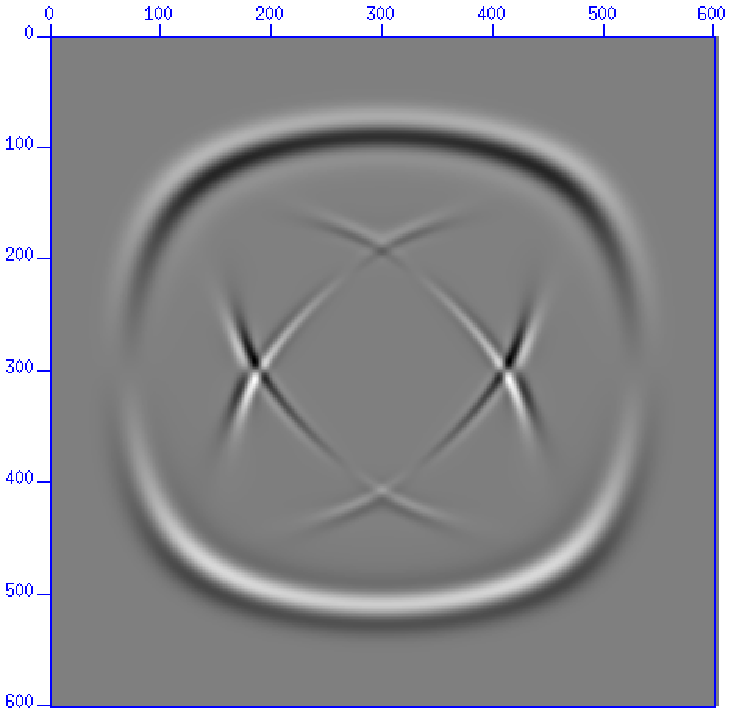
\includegraphics[width=6.5cm,height=6.5cm]{Figs/snap}
\caption[Exemplo de figura simples (texto do índice).]{Exemplo de figura simples:
modelagem elástica de um meio anisotrópico.}
\label{fig:caption1}
\end{figure}

Exemplo de utilização de figuras múltiplas é apresentado na Figura~\ref{fig:cc}
abaixo. Podemos referenciar cada uma das figuras, por exemplo a Figura~\ref{fig:cc_nr} ou
a Figura~\ref{fig:cc_cerjan}.
\begin{figure}[hbt]
\centering \subfigure[Condição de contorno não reflexiva
(CCNR).]{\label{fig:cc_nr}
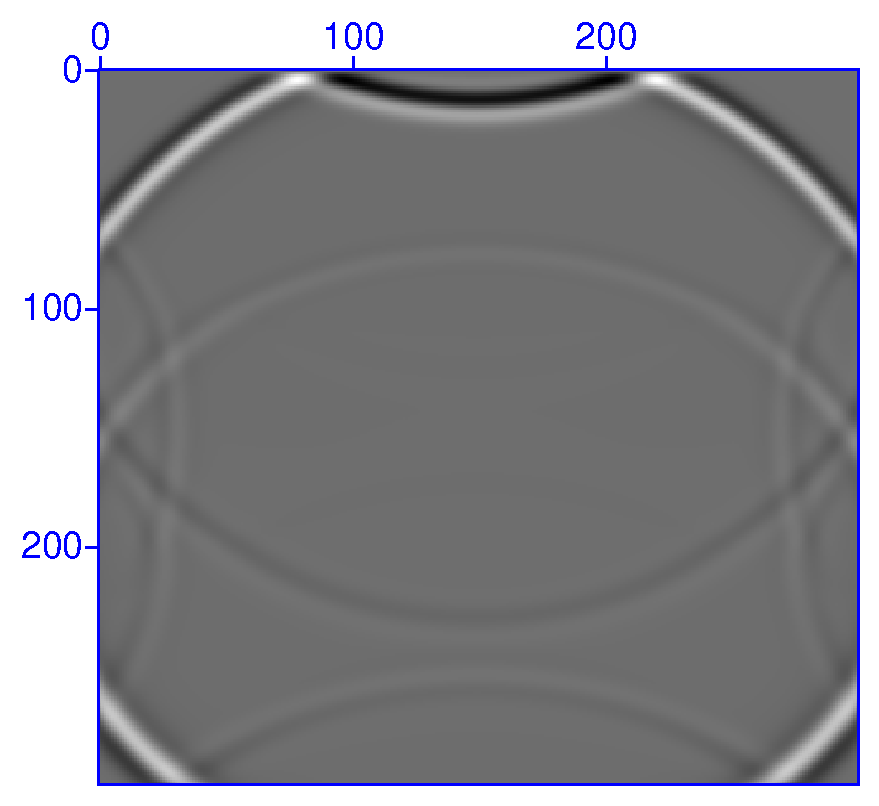
\includegraphics[width=6.5cm,height=6.5cm]
{Figs/cc_nr}} \qquad \subfigure[Camadas de amortecimento +
CCNR.]{\label{fig:cc_cerjan}
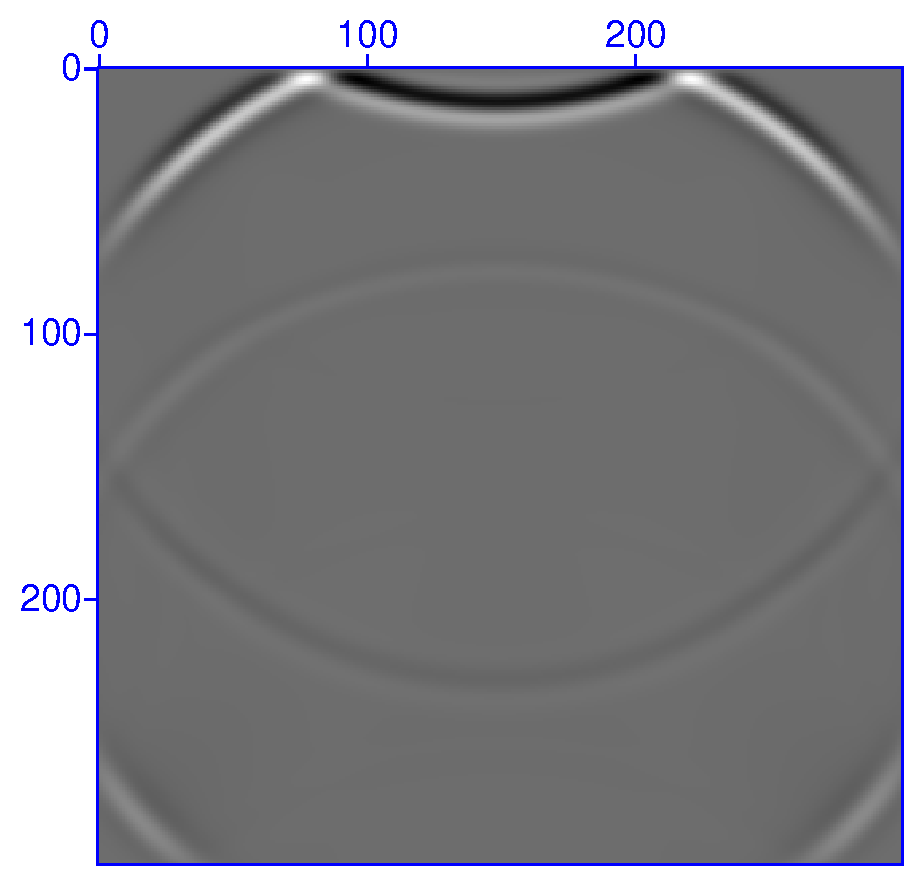
\includegraphics[width=6.5cm,height=6.5cm]{Figs/cerjan}}
\caption[Exemplo de múltiplas figuras (texto do índice).]{Exemplo de múltiplas
figuras: modelagem
acústica mostrando efeito da aplicação da CCNR e camadas de amortecimento
aplicadas nas bordas (menos na superfície). Aplica-se em (a) as CCNR de
Reynolds e em (b) as camadas de amortecimento mais CCNR de Reynolds.}
\label{fig:cc}
\end{figure}

Repare para que o exemplo acima funcione corretamente, é necessário a utilização do pacote``\verb|\usepackage{subfigure}|'', declarado no preambulo do documento principal. Para tal, este pacete deve estar instalado no LaTex utilizado para processar o documento. Indicamos a utilização do MikTex (gratuito) mais atual com editor WinEdt (pago).
  \chapter{Título capítulo 4}

  \chapter{Resultados e Discussões}

  \chapter{Conclusões}


  \backmatter
  \bibliographystyle{on-plain} %usar em conjnunto com o estilo de citações por ordem alfabética (defaut da classe ONTeX)
%  \bibliographystyle{on-unsrt} %usar em conjnunto com o estilo de citações por lista em ordem de ocorrência no texto (utilizar a opção "numbers" na classe ONTeX)
  \bibliography{thesis}

  \appendix
  \chapter{Algumas Demonstrações}

Aqui devem entrar demonstrações mais longas, revisões de conceitos mais básicos
ou qualquer detalhe pertinente que não seja adequado para o corpo da
dissertação/tese.

\end{document} 